\documentclass[12pt,letterpaper]{article}

%Packages
% \usepackage{textcomp}
% \usepackage{latexsym}
% \usepackage{url}
% \usepackage{epsfig}
% \usepackage{graphicx}
% \usepackage{amssymb}
% \usepackage{amsmath}
% \usepackage{mathtools}
% \usepackage{bm}
% \usepackage{array}
% \usepackage[version=3]{mhchem}
% \usepackage{ifthen}
% \usepackage{caption}
% \usepackage{amsthm}
% \usepackage{amstext}
% \usepackage{enumerate}
% \usepackage[osf]{mathpazo}
% \usepackage{dcolumn}

\usepackage{hyperref}
\usepackage{lineno}
\usepackage{pdflscape}
\usepackage{mathtools}
\usepackage[osf]{mathpazo}
\usepackage{fullpage}
% \usepackage{float}

\pagenumbering{arabic}


%---------------------------------------------
%
%       START
%
%---------------------------------------------

\begin{document}
%Running head
\begin{flushright}
Version dated: \today
\end{flushright}

\bigskip
\medskip
\begin{center}

\noindent{\Large \bf Innovation and elaboration on the avian tree of life - supplementary materials}
\bigskip

\noindent {\normalsize \sc Thomas Guillerme$^{1,*}$, Natalie Cooper$^{2}$, Andrew P. Beckerman$^{1}$, and Gavin H. Thomas$^{1,3}$}\\
\noindent {\small \it 
$^1$School of Biosciences, University of Sheffield, Sheffield, S10 2TN, United Kingdom.\\
$^2$Natural History Museum, Cromwell Road, London, SW7 5BD, United Kingdom.\\
$^3$Bird Group, Department of Life Sciences, the Natural History Museum at Tring, Tring, United Kingdom.\\}

\end{center}
\medskip
\noindent{*\bf Corresponding author.} \textit{guillert@tcd.ie}\\ 
\vspace{1in}

%Line numbering
\modulolinenumbers[1]
\linenumbers

\noindent (Keywords: )\\

\vspace{1.5in}

\newpage 

%---------------------------------------------
%
%       INTRODUCTION
%
%---------------------------------------------


\section{Supplementary material 1: glossary}

\begin{table}[ht]
\centering
\scriptsize
\begin{tabular}{llll}
  \hline
Term in this paper          & evolutionary biology definition & mathematics definition \\
  \hline
clade                       & a monophyletic group of species & a distance matrix associated with a subset of the \textbf{shapespace} \\ 
clade's major axis          & the \textbf{line of least resistance} specific to a clade & the first \textbf{eigenvector} of a \textbf{clade}'s \textbf{variance-covariance} matrix &  \\ 
eigenvector                 & one evolutionary \textbf{line of least resistance} for a clade & one of the vectors (direction) defining a \textbf{variance-covariance} matrix \\
elaboration                 & morphological score of a \textbf{species} or a \textbf{clade} in relation to a \textbf{line of least resistance} of reference & the \textbf{projection} of a \textbf{species} or a \textbf{clade} onto the first \textbf{eigenvector} of a \textbf{variance-covariance} matrix \\
family                      & a specific \textbf{clade} level (nested within \textbf{sub-orders}) & a distance matrix \\
higher taxa                 & a higher \textbf{clade} level & a distance matrix associated with a subset of the \textbf{shapespace} \\
innovation                  & morphological score of a \textbf{species} or a \textbf{clade} in relation to a \textbf{line of least resistance} of reference & the \textbf{rejection} of a \textbf{species} or a \textbf{clade} away from the first \textbf{eigenvector} of a \textbf{variance-covariance} matrix \\
lines of least resistance   & the major evolutionary ``direction'' of traits co-evolution & the first \textbf{eigenvector} or a \textbf{variance-covariance} matrix \\
macroevolution              & evolution above the species level & analyses using a portion of the entire shapespace \\
major axis                  & one of the ``directions'' of traits co-evolution & an \textbf{eigenvector} or a \textbf{variance-covariance} matrix; this can be represented as the longest orthogonal lines of an ellipse \\
megaevolution               & evolution above the \textbf{clade} level - here arbitrarily defined at the whole \textbf{phylogeny} level (i.e. all the birds) & analyses using the entire shapespace \\
order                       & a specific \textbf{clade} level (nested within \textbf{super-orders}) & a distance matrix associated with a subset of the \textbf{shapespace} \\
phylogenetic major axis     & the \textbf{line of least resistance} for the whole \textbf{phylogeny} & the first \textbf{eigenvector} of the whole \textbf{phylogeny}'s \textbf{variance-covariance} matrix \\
phylogeny                   & the relationships between all the \textbf{species} and their respective \textbf{clades} used in this analysis & a distance matrix associated with the whole \textbf{shapespace} \\
projection                  & the \textbf{elaboration} score of \textbf{species} or a \textbf{clade} & the position of a \textbf{species} or a \textbf{clade} onto an \textbf{eigenvector}\\
rejection                   & the \textbf{innovation} score of \textbf{species} or a \textbf{clade} & the distance of a \textbf{species} or a \textbf{clade} away from an \textbf{eigenvector} \\
residual                    & the variation in the \textbf{shapespace} not explained by the \textbf{phylogeny} or a \textbf{clade} & the error term in the pGLMM not explained by the random error terms (\textbf{phylogeny} and \textbf{clade}) \\
shapespace                  & all the observed morphological combination of the 8748 \textbf{species} of birds & a matrix where each columns are traits (or a transformation thereof, here they are principal components) and each rows are observations (here \textbf{species}). \\
species                     & the lowest evolutionary units in our analysis & rows in the \textbf{shapespace} matrix \\
sub-orders                  & a specific \textbf{clade} level (nested within \textbf{orders}) & a distance matrix associated with a subset of the \textbf{shapespace} \\
super-order                 & a specific \textbf{clade} level (the first nested level within the whole \textbf{phylogeny}) & a distance matrix associated with a subset of the \textbf{shapespace} \\
variance-covariance         & the traits co variation in the \textbf{shapespace} & the variation of the dimension within the \textbf{shapespace} taking into account the distance matrix between the observations (the \textbf{phylogeny} or the \textbf{clades}) \\

\end{tabular}
\caption{Glossary of some specific terms in this manuscript}
\label{tab_glossary}
\end{table}




\section{Supplementary material 2: additional results}

\begin{figure}[!htbp]
\centering
   \includegraphics[width=0.9\textwidth]{Figures/cheat_sheet.pdf}
\caption{\scriptsize Relation between the figures in the main text.
The top left panel represents the two first dimensions of the 8 dimensional trait space with all bird beaks represented as grey circles and the Palaeognathes as red ones.
The grey ellipse represents the average posterior variance covariance matrix (VCV) from the general phylogenetic random term of the MCMCglmm model (i.e. the overall phylogenetic axis of main variation).
Species aligned with this axis tend to be elaborators at the mega-evolutionary level and species going away from that line are innovators at the mega-evolutionary level.
The red ellipse and axis represents the average posterior VCV for the Palaeognathes only.
Species position on this axis elaborate and innovate at the macro-evolutionary level.
On the top right panel (Figure 1 in the main text), we measured the elaboration and innovation at the entire clade level (cf. at the species level below).
The ellipses are a scaled and centered in space representation of the group’s VCV ellipse relative to the overall phylogenetic one with a the relative length of the ellipse on each dimension represented on the barplots.
The clade's innovation and elaboration scores are measured by projecting the clade's major axis onto the phylogenetic one and measuring the projection (elaboration) and rejection (innovation) as mentioned above.
The distribution of innovation and elaboration scores comes from the projection of the 4000 pairs of posterior VCVs.
On the bottom right panel (Figure 3 in the main text), we measured the position of each species in terms of elaboration and innovation.
A species elaboration score is their projection onto the phylogenetics' VCV major axis (i.e. their position on that axis) whereas their innovation score is their rejection from it (i.e. their distance away from that axis).}
\label{Fig:cheat_sheet}
\end{figure}


\begin{figure}[!htbp]
\centering
   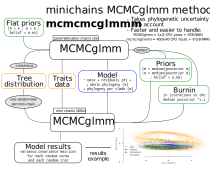
\includegraphics[width=0.9\textwidth]{Figures/mini-chains_diagram.pdf}
\caption{mcmcmcglmmm: mini-chains MCMCglmm method diagram}
\label{Fig:mcmcmcglmm}
\end{figure}


\begin{figure}[!htbp]
\centering
   \includegraphics[width=0.9\textwidth]{Figures/axis_selection.pdf}
\caption{variance and cumulative variance for each 8 axis per super-order.}
\label{Fig:axes_variance}
\end{figure}



\begin{figure}[!htbp]
\centering
   \includegraphics[width=0.5\textwidth]{Figures/parameters_ESS_all_birds.pdf}
\caption{Histogram of the effective sample sizes (ESS) for each class of parameters in the MCMCglmm model for all birds for the 4000 posteriors. \textbf{solution} is the solution of the model; \textbf{Gcovariance} are the covariances for the random terms (the phylogeny and the clades); \textbf{Rcovariance} are the residuals error term.}
\label{Fig:model_ess_all_birds}
\end{figure}

\begin{figure}[!htbp]
\centering
   \includegraphics[width=0.5\textwidth]{Figures/parameters_ESS_passeriformes.pdf}
\caption{Histogram of the effective sample sizes (ESS) for each class of parameters in the MCMCglmm model for the passeriformes for the 1870 posteriors. \textbf{solution} is the solution of the model; \textbf{Gcovariance} are the covariances for the random terms (the phylogeny and the clades); \textbf{Rcovariance} are the residuals error term.}
\label{Fig:model_ess_passeriformes}
\end{figure}


\begin{landscape}
% latex table generated in R 4.2.2 by xtable 1.8-4 package
% Wed Nov  9 11:43:10 2022
\begin{table}[ht]
\centering
\begin{tabular}{rrrrrrrrrrrrrrrrrrr}
  \hline
 & PC1.var & PC1.sum & PC2.var & PC2.sum & PC3.var & PC3.sum & PC4.var & PC4.sum & PC5.var & PC5.sum & PC6.var & PC6.sum & PC7.var & PC7.sum & PC8.var & PC8.sum & PC9.var & PC9.sum \\ 
  \hline
no clade & 0.504 & 0.504 & 0.339 & 0.843 & 0.078 & 0.921 & 0.025 & 0.945 & 0.015 & 0.961 & 0.008 & 0.969 & 0.010 & 0.979 & 0.006 & 0.984 & 0.003 & 0.987 \\ 
  Aequornithes & 0.384 & 0.384 & 0.375 & 0.759 & 0.075 & 0.834 & 0.030 & 0.864 & 0.020 & 0.884 & 0.011 & 0.895 & 0.047 & 0.942 & 0.017 & 0.959 & 0.014 & 0.972 \\ 
  Columbimorphae & 0.293 & 0.293 & 0.456 & 0.750 & 0.093 & 0.843 & 0.040 & 0.883 & 0.016 & 0.899 & 0.040 & 0.938 & 0.019 & 0.957 & 0.005 & 0.962 & 0.006 & 0.968 \\ 
  Eurypygimorphae & 0.440 & 0.440 & 0.146 & 0.586 & 0.266 & 0.852 & 0.005 & 0.857 & 0.038 & 0.896 & 0.039 & 0.934 & 0.026 & 0.960 & 0.003 & 0.964 & 0.003 & 0.966 \\ 
  Galloanserae & 0.253 & 0.253 & 0.401 & 0.653 & 0.141 & 0.795 & 0.118 & 0.912 & 0.032 & 0.944 & 0.011 & 0.955 & 0.009 & 0.964 & 0.010 & 0.974 & 0.004 & 0.978 \\ 
  Mirandornithes & 0.124 & 0.124 & 0.337 & 0.461 & 0.040 & 0.501 & 0.313 & 0.814 & 0.089 & 0.902 & 0.006 & 0.908 & 0.057 & 0.965 & 0.017 & 0.982 & 0.004 & 0.986 \\ 
  Otidimorphae & 0.401 & 0.401 & 0.396 & 0.797 & 0.090 & 0.887 & 0.051 & 0.938 & 0.013 & 0.951 & 0.021 & 0.972 & 0.007 & 0.979 & 0.004 & 0.983 & 0.003 & 0.986 \\ 
  Paleognathae & 0.363 & 0.363 & 0.402 & 0.766 & 0.133 & 0.899 & 0.027 & 0.926 & 0.018 & 0.944 & 0.028 & 0.972 & 0.008 & 0.980 & 0.002 & 0.982 & 0.003 & 0.985 \\ 
  Strisores & 0.712 & 0.712 & 0.226 & 0.938 & 0.024 & 0.961 & 0.024 & 0.985 & 0.003 & 0.988 & 0.004 & 0.992 & 0.002 & 0.994 & 0.002 & 0.996 & 0.001 & 0.997 \\ 
  Telluraves & 0.511 & 0.511 & 0.341 & 0.851 & 0.073 & 0.924 & 0.021 & 0.945 & 0.014 & 0.959 & 0.014 & 0.974 & 0.008 & 0.982 & 0.004 & 0.986 & 0.003 & 0.989 \\ 
  Entire space & 0.554 & 0.554 & 0.297 & 0.851 & 0.066 & 0.917 & 0.028 & 0.945 & 0.016 & 0.962 & 0.011 & 0.973 & 0.009 & 0.982 & 0.004 & 0.987 & 0.003 & 0.989 \\ 
   \hline
\end{tabular}
\caption{Variance per axis and per group in the shape space. The "no clade" group contains birds not attributed to any of the other groups (i.e. from a clade with less than 15 species).} 
\label{tab_variance_per_axis}
\end{table}

\end{landscape}


% latex table generated in R 4.2.1 by xtable 1.8-4 package
% Thu Aug  4 16:49:31 2022
\begin{table}[ht]
\centering
\scriptsize
\begin{tabular}{llrrrrrrrr}
  \hline
Group & Comparison & n & ellipse sd & orthogonality & 2.5\% & 97.5\% & Post. prob. & 2.5\% & 97.5\% \\ 
  \hline
Aequornithes & phylogeny &  308 & 15.465 & 0.710 & 0.219 & 0.988 & 0.811 & 0.802 & 0.818 \\ 
  Columbimorphae & phylogeny &  285 & 5.916 & 0.884 & 0.564 & 0.995 & 0.998 & 0.997 & 0.999 \\ 
  Galloanserae & phylogeny &  421 & 13.489 & 0.800 & 0.369 & 0.992 & 0.832 & 0.826 & 0.838 \\ 
  Mirandornithes & phylogeny &   24 & 20.870 & 0.839 & 0.448 & 0.992 & 0.496 & 0.489 & 0.505 \\ 
  Otidimorphae & phylogeny &  181 & 16.800 & 0.680 & 0.291 & 0.983 & 0.795 & 0.788 & 0.802 \\ 
  Paleognathae & phylogeny &   52 & 20.728 & 0.718 & 0.264 & 0.985 & 0.803 & 0.797 & 0.810 \\ 
  Strisores & phylogeny &  370 & 16.237 & 0.787 & 0.469 & 0.986 & 0.992 & 0.990 & 0.994 \\ 
  Telluraves & phylogeny & 6604 & 14.339 & 0.730 & 0.294 & 0.988 & 0.662 & 0.655 & 0.672 \\ 
  Accipitriformes & phylogeny &  240 & 5.044 & 0.906 & 0.706 & 0.996 & 1.000 & 1.000 & 1.000 \\ 
  Anseriformes & phylogeny &  156 & 13.546 & 0.743 & 0.167 & 0.989 & 0.781 & 0.773 & 0.790 \\ 
  Apodiformes & phylogeny &  331 & 18.307 & 0.684 & 0.326 & 0.971 & 0.887 & 0.881 & 0.894 \\ 
  Bucerotiformes & phylogeny &   66 & 4.651 & 0.857 & 0.542 & 0.993 & 0.983 & 0.980 & 0.985 \\ 
  Caprimulgiformes & phylogeny &   23 & 11.555 & 0.847 & 0.533 & 0.992 & 0.938 & 0.934 & 0.943 \\ 
  Charadriiformes & phylogeny &  359 & 5.632 & 0.331 & 0.148 & 0.592 & 0.915 & 0.909 & 0.920 \\ 
  Ciconiiformes & phylogeny &   19 & 20.915 & 0.839 & 0.459 & 0.992 & 0.519 & 0.509 & 0.528 \\ 
  Columbiformes & phylogeny &  266 & 3.975 & 0.896 & 0.649 & 0.996 & 1.000 & 1.000 & 1.000 \\ 
  Coraciiformes & phylogeny &  149 & 17.618 & 0.358 & 0.196 & 0.603 & 0.980 & 0.976 & 0.983 \\ 
  Cuculiformes & phylogeny &  134 & 18.927 & 0.603 & 0.217 & 0.970 & 0.753 & 0.746 & 0.761 \\ 
  Falconiformes & phylogeny &   63 & 12.521 & 0.851 & 0.520 & 0.993 & 0.979 & 0.977 & 0.982 \\ 
  Galliformes & phylogeny &  265 & 1.416 & 0.894 & 0.694 & 0.995 & 1.000 & 1.000 & 1.000 \\ 
  Gruiformes & phylogeny &  138 & 7.922 & 0.543 & 0.215 & 0.894 & 0.948 & 0.944 & 0.953 \\ 
  Musophagiformes & phylogeny &   22 & 11.601 & 0.898 & 0.581 & 0.996 & 0.922 & 0.916 & 0.927 \\ 
  Otidiformes & phylogeny &   25 & 17.148 & 0.706 & 0.271 & 0.983 & 0.482 & 0.473 & 0.490 \\ 
  Passeriformes & phylogeny & 5229 & 11.642 & 0.428 & 0.189 & 0.650 & 1.000 & 0.999 & 1.000 \\ 
  Pelecaniformes & phylogeny &  103 & 28.435 & 0.537 & 0.284 & 0.937 & 0.747 & 0.741 & 0.755 \\ 
  Piciformes & phylogeny &  390 & 15.366 & 0.460 & 0.216 & 0.684 & 1.000 & 0.999 & 1.000 \\ 
  Podicipediformes & phylogeny &   18 & 20.335 & 0.828 & 0.453 & 0.993 & 0.491 & 0.482 & 0.500 \\ 
  Procellariiformes & phylogeny &  112 & 13.408 & 0.529 & 0.241 & 0.949 & 0.608 & 0.600 & 0.617 \\ 
  Psittaciformes & phylogeny &  341 & 12.975 & 0.572 & 0.433 & 0.755 & 1.000 & 1.000 & 1.000 \\ 
  Pterocliformes & phylogeny &   16 & 21.382 & 0.834 & 0.459 & 0.994 & 0.507 & 0.500 & 0.518 \\ 
  Sphenisciformes & phylogeny &   17 & 21.149 & 0.809 & 0.415 & 0.991 & 0.501 & 0.490 & 0.509 \\ 
  Strigiformes & phylogeny &   76 & 2.241 & 0.921 & 0.721 & 0.996 & 1.000 & 1.000 & 1.000 \\ 
  Suliformes & phylogeny &   52 & 7.537 & 0.745 & 0.437 & 0.976 & 0.994 & 0.993 & 0.996 \\ 
  Tinamiformes & phylogeny &   41 & 18.518 & 0.805 & 0.331 & 0.991 & 0.721 & 0.711 & 0.729 \\ 
  Trogoniformes & phylogeny &   41 & 9.463 & 0.882 & 0.593 & 0.995 & 0.997 & 0.996 & 0.999 \\ 
  Procellariiformes & Aequornithes &  112 & 13.408 & 0.677 & 0.263 & 0.986 & 0.699 & 0.690 & 0.707 \\ 
  Sphenisciformes & Aequornithes &   17 & 21.149 & 0.744 & 0.348 & 0.988 & 0.414 & 0.406 & 0.423 \\ 
  Ciconiiformes & Aequornithes &   19 & 20.915 & 0.790 & 0.365 & 0.987 & 0.436 & 0.426 & 0.444 \\ 
  Pelecaniformes & Aequornithes &  103 & 28.435 & 0.541 & 0.196 & 0.968 & 0.675 & 0.666 & 0.683 \\ 
  Suliformes & Aequornithes &   52 & 7.537 & 0.299 & 0.128 & 0.875 & 0.761 & 0.754 & 0.769 \\ 
  Columbiformes & Columbimorphae &  266 & 3.975 & 0.182 & 0.079 & 0.424 & 0.638 & 0.630 & 0.647 \\ 
  Pterocliformes & Columbimorphae &   16 & 21.382 & 0.801 & 0.396 & 0.993 & 0.464 & 0.454 & 0.473 \\ 
  Galliformes & Galloanserae &  265 & 1.416 & 0.327 & 0.146 & 0.905 & 1.000 & 1.000 & 1.000 \\ 
  Anseriformes & Galloanserae &  156 & 13.546 & 0.499 & 0.206 & 0.963 & 0.599 & 0.591 & 0.606 \\ 
  Podicipediformes & Mirandornithes &   18 & 20.335 & 0.552 & 0.170 & 0.972 & 0.492 & 0.483 & 0.500 \\ 
  Otidiformes & Otidimorphae &   25 & 17.148 & 0.608 & 0.208 & 0.980 & 0.397 & 0.390 & 0.406 \\ 
  Cuculiformes & Otidimorphae &  134 & 18.927 & 0.486 & 0.173 & 0.959 & 0.517 & 0.510 & 0.527 \\ 
  Musophagiformes & Otidimorphae &   22 & 11.601 & 0.487 & 0.181 & 0.963 & 0.590 & 0.582 & 0.598 \\ 
  Tinamiformes & Paleognathae &   41 & 18.518 & 0.455 & 0.145 & 0.964 & 0.440 & 0.433 & 0.450 \\ 
  Caprimulgiformes & Strisores &   23 & 11.555 & 0.327 & 0.152 & 0.858 & 0.516 & 0.506 & 0.524 \\ 
  Apodiformes & Strisores &  331 & 18.307 & 0.340 & 0.141 & 0.797 & 0.529 & 0.519 & 0.536 \\ 
  Trogoniformes & Telluraves &   41 & 9.463 & 0.500 & 0.200 & 0.963 & 0.881 & 0.874 & 0.887 \\ 
  Bucerotiformes & Telluraves &   66 & 4.651 & 0.489 & 0.181 & 0.959 & 0.820 & 0.814 & 0.826 \\ 
  Coraciiformes & Telluraves &  149 & 17.618 & 0.676 & 0.343 & 0.983 & 0.999 & 0.998 & 1.000 \\ 
  Piciformes & Telluraves &  390 & 15.366 & 0.605 & 0.226 & 0.978 & 1.000 & 0.999 & 1.000 \\ 
  Strigiformes & Telluraves &   76 & 2.241 & 0.523 & 0.207 & 0.962 & 1.000 & 0.999 & 1.000 \\ 
  Accipitriformes & Telluraves &  240 & 5.044 & 0.482 & 0.169 & 0.961 & 0.976 & 0.974 & 0.980 \\ 
  Falconiformes & Telluraves &   63 & 12.521 & 0.523 & 0.206 & 0.964 & 0.839 & 0.831 & 0.846 \\ 
  Psittaciformes & Telluraves &  341 & 12.975 & 0.648 & 0.275 & 0.982 & 1.000 & 0.999 & 1.000 \\ 
  Passeriformes & Telluraves & 5229 & 11.642 & 0.634 & 0.274 & 0.980 & 1.000 & 1.000 & 1.000 \\ 
  Corvides & Passeriformes &  609 & 16.462 & 0.195 & 0.097 & 0.495 & 0.546 & 0.530 & 0.561 \\ 
  Meliphagoidea & Passeriformes &  214 & 19.362 & 0.248 & 0.120 & 0.832 & 0.524 & 0.509 & 0.542 \\ 
  Muscicapida & Passeriformes &  702 & 16.961 & 0.354 & 0.101 & 0.798 & 0.681 & 0.663 & 0.697 \\ 
  Passerida & Passeriformes & 1492 & 3.448 & 0.370 & 0.203 & 0.542 & 1.000 & 0.998 & 1.000 \\ 
  Suboscines & Passeriformes &  978 & 13.676 & 0.455 & 0.173 & 0.889 & 0.796 & 0.785 & 0.814 \\ 
  Sylviida & Passeriformes & 1131 & 16.555 & 0.474 & 0.128 & 0.947 & 0.527 & 0.510 & 0.548 \\ 
  Aegithaloidea & Passeriformes &  105 & 24.869 & 0.324 & 0.155 & 0.899 & 0.447 & 0.431 & 0.462 \\ 
  Bombycilloidea & Passeriformes &  112 & 10.938 & 0.404 & 0.179 & 0.728 & 0.834 & 0.818 & 0.850 \\ 
  Cisticolidae & Passeriformes &  141 & 14.966 & 0.459 & 0.173 & 0.905 & 0.519 & 0.504 & 0.533 \\ 
  Corvoidea & Passeriformes &  248 & 3.303 & 0.499 & 0.343 & 0.672 & 1.000 & 1.000 & 1.000 \\ 
  Emberizoidea & Passeriformes &  752 & 16.601 & 0.455 & 0.210 & 0.932 & 0.730 & 0.716 & 0.746 \\ 
  Eurylaimides & Passeriformes &   51 & 22.653 & 0.165 & 0.075 & 0.423 & 0.440 & 0.423 & 0.454 \\ 
  Fringillidae & Passeriformes &   87 & 3.730 & 0.428 & 0.198 & 0.751 & 0.926 & 0.914 & 0.938 \\ 
  Furnariida & Passeriformes &  488 & 6.684 & 0.384 & 0.198 & 0.640 & 0.904 & 0.892 & 0.915 \\ 
  Hirundinidae & Passeriformes &   77 & 10.776 & 0.691 & 0.447 & 0.967 & 0.950 & 0.942 & 0.957 \\ 
  Locustelloidea & Passeriformes &  106 & 22.109 & 0.339 & 0.117 & 0.892 & 0.481 & 0.465 & 0.497 \\ 
  Malaconotoidea & Passeriformes &  205 & 19.275 & 0.495 & 0.283 & 0.838 & 0.883 & 0.873 & 0.891 \\ 
  Meliphagoidea & Passeriformes &  214 & 19.362 & 0.239 & 0.106 & 0.741 & 0.524 & 0.504 & 0.545 \\ 
  Motacillidae & Passeriformes &   58 & 16.078 & 0.486 & 0.186 & 0.918 & 0.638 & 0.625 & 0.653 \\ 
  Muscicapoidea & Passeriformes &  576 & 17.136 & 0.318 & 0.113 & 0.624 & 0.763 & 0.751 & 0.778 \\ 
  Nectariniidae & Passeriformes &  166 & 19.789 & 0.222 & 0.109 & 0.427 & 0.651 & 0.638 & 0.669 \\ 
  Orioloidea & Passeriformes &   54 & 21.510 & 0.466 & 0.147 & 0.972 & 0.500 & 0.484 & 0.520 \\ 
  Paridae & Passeriformes &   69 & 8.747 & 0.559 & 0.275 & 0.851 & 0.937 & 0.927 & 0.943 \\ 
  Passeridae & Passeriformes &   39 & 19.891 & 0.525 & 0.146 & 0.969 & 0.418 & 0.405 & 0.433 \\ 
  Petroicidae & Passeriformes &   35 & 31.236 & 0.484 & 0.170 & 0.975 & 0.401 & 0.387 & 0.419 \\ 
  PloceidaeEstrildidae & Passeriformes &  261 & 6.009 & 0.896 & 0.627 & 0.995 & 1.000 & 0.999 & 1.000 \\ 
  Pycnonotidae & Passeriformes &  123 & 17.818 & 0.229 & 0.117 & 0.581 & 0.521 & 0.506 & 0.540 \\ 
  Sylvioidea & Passeriformes &  403 & 12.158 & 0.405 & 0.157 & 0.944 & 0.572 & 0.557 & 0.589 \\ 
  Tyrannida & Passeriformes &  439 & 26.513 & 0.466 & 0.181 & 0.936 & 0.586 & 0.570 & 0.607 \\ 
  Orioloidea & Corvides &   54 & 21.510 & 0.502 & 0.150 & 0.968 & 0.487 & 0.469 & 0.502 \\ 
  Corvoidea & Corvides &  248 & 3.303 & 0.464 & 0.171 & 0.761 & 0.995 & 0.990 & 0.998 \\ 
  Malaconotoidea & Corvides &  205 & 19.275 & 0.556 & 0.283 & 0.893 & 0.892 & 0.881 & 0.903 \\ 
  Bombycilloidea & Muscicapida &  112 & 10.938 & 0.260 & 0.093 & 0.742 & 0.572 & 0.550 & 0.593 \\ 
  Muscicapoidea & Muscicapida &  576 & 17.136 & 0.271 & 0.085 & 0.796 & 0.578 & 0.553 & 0.591 \\ 
  Nectariniidae & Passerida &  166 & 19.789 & 0.464 & 0.278 & 0.719 & 0.960 & 0.952 & 0.967 \\ 
  PloceidaeEstrildidae & Passerida &  261 & 6.009 & 0.605 & 0.369 & 0.834 & 0.991 & 0.986 & 0.995 \\ 
  Emberizoidea & Passerida &  752 & 16.601 & 0.765 & 0.271 & 0.984 & 0.885 & 0.875 & 0.898 \\ 
  Motacillidae & Passerida &   58 & 16.078 & 0.756 & 0.239 & 0.987 & 0.823 & 0.810 & 0.839 \\ 
  Passeridae & Passerida &   39 & 19.891 & 0.668 & 0.225 & 0.986 & 0.524 & 0.506 & 0.540 \\ 
  Eurylaimides & Suboscines &   51 & 22.653 & 0.495 & 0.222 & 0.928 & 0.909 & 0.895 & 0.922 \\ 
  Tyrannida & Suboscines &  439 & 26.513 & 0.404 & 0.134 & 0.956 & 0.479 & 0.458 & 0.494 \\ 
  Furnariida & Suboscines &  488 & 6.684 & 0.245 & 0.100 & 0.764 & 0.695 & 0.679 & 0.709 \\ 
  Paridae & Sylviida &   69 & 8.747 & 0.388 & 0.151 & 0.934 & 0.788 & 0.771 & 0.802 \\ 
  Locustelloidea & Sylviida &  106 & 22.109 & 0.483 & 0.168 & 0.930 & 0.664 & 0.646 & 0.682 \\ 
  Aegithaloidea & Sylviida &  105 & 24.869 & 0.530 & 0.177 & 0.967 & 0.642 & 0.626 & 0.661 \\ 
  Hirundinidae & Sylviida &   77 & 10.776 & 0.522 & 0.272 & 0.956 & 0.857 & 0.842 & 0.867 \\ 
  Pycnonotidae & Sylviida &  123 & 17.818 & 0.558 & 0.172 & 0.979 & 0.842 & 0.830 & 0.860 \\ 
  Sylvioidea & Sylviida &  403 & 12.158 & 0.444 & 0.132 & 0.963 & 0.575 & 0.557 & 0.593 \\ 
  Cisticolidae & Sylviida &  141 & 14.966 & 0.477 & 0.145 & 0.955 & 0.531 & 0.516 & 0.553 \\ 
  Fringillidae & Sylviida &   87 & 3.730 & 0.718 & 0.179 & 0.988 & 0.964 & 0.955 & 0.973 \\ 
   \hline
\end{tabular}
\caption{Posterior variance-covariance ellipses results for each clade compared to their parent clade or their parent parents clade (Comparison). n = the number of species per group. sd = the standard deviation of the ellipses orientation (across the posterior distribution). orthogonality = the degree of right angle for each group compared to their parent or parent's group (0 = parellel, 1 = orthogonal). Post. prob = the posterior probability of the orthogonality in the focal group being different from the comparison one (the 95\% CI is from the randomised posterior probabilities).} 
\label{tab_ortho_results}
\end{table}



\section{Supplementary material 3: Passeriformes results}

\begin{figure}[!htbp]
\centering
   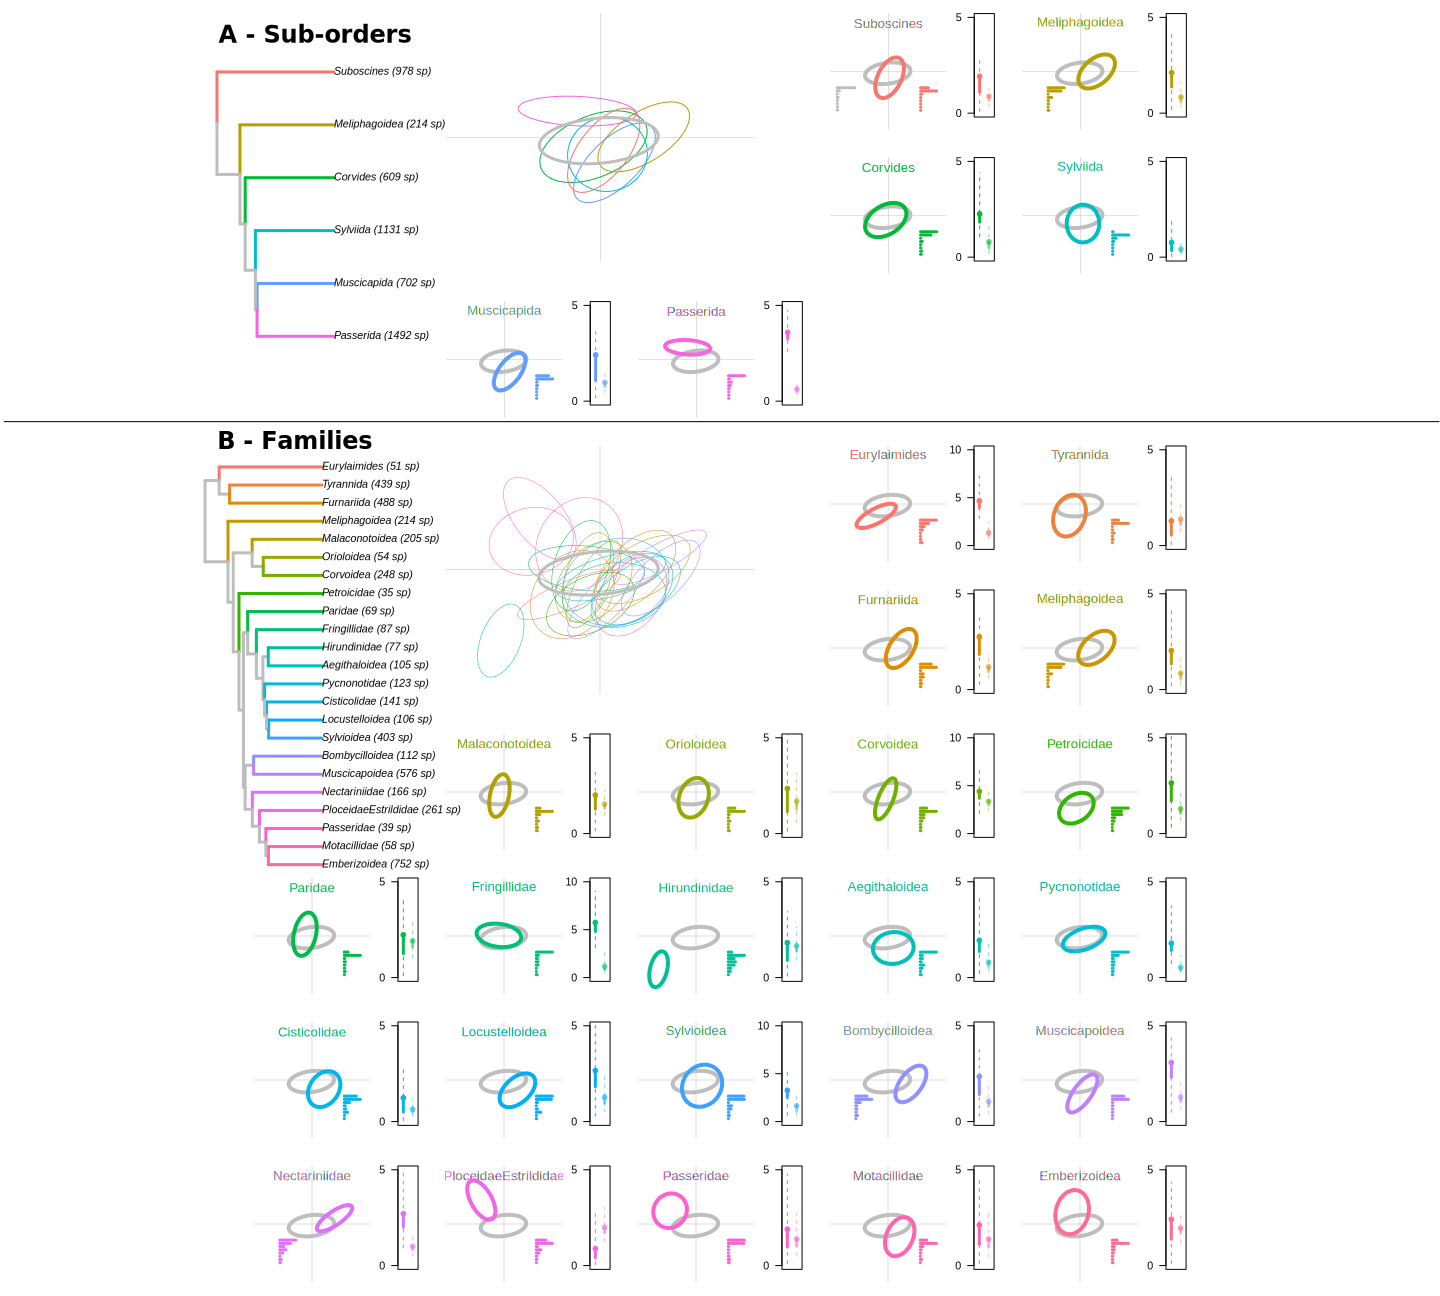
\includegraphics[width=1\textwidth]{Figures/ellipses_passeriformes.pdf}
\caption{Elaboration and innovation at the group level for each passeriformes sub-orders and families. See the caption of figure 1 in the main text for details.}
\label{fig_ellipses_passeriformes}
\end{figure}

\begin{figure}[!htbp]
\centering
   \includegraphics[width=0.9\textwidth]{Figures/orthogonality_results_passeriformes.pdf}
\caption{Posterior results showing the orientation of phenotypic evolution (orthogonality) for each passeriformes sub-orders and families. See the caption of figure 2 in the main text for details.}
\label{fig_orthogonality_passeriformes}
\end{figure}


\begin{figure}[!htbp]
\centering
    \includegraphics[width=0.9\textwidth]{Figures/InnovElabTree_passerine_supplement.pdf}
\caption{Passeriformes phylogeny coloured by beak shape innovation and elaboration level. See the caption of figure 3 in the main text for details.}
\label{fig_phylogeny_passeriformes}
\end{figure}

\newpage

\section{Supplementary materials 4: detailed projection and rejection operations}
\label{supp_projection}

The following section contains the detailed definition and procedure of how we measured elaboration and innovation

We can define the major axis from the variance-covariance matrices and then project and reject each element of interest in the space onto this axis.
The following steps are generalised to $n$ dimensions and detailed below (as well as the algorithm used in \texttt{dispRity} \cite{dispRity} to perform the transformations):

\subsection{Defining the major axis}

For $O_{n}$, the unit hypersphere matrix of $n$ dimensions and a radius composed of the two identity matrices $I_{n}$ and $-I_{n}$ so that: 

\begin{equation}
O_{n} = 
    \begin{pmatrix}
        1 & 0 & \cdots & 0 \\
        0 & 1 & \cdots & 0 \\
        \vdots  & \vdots  & \ddots & \vdots  \\
        0 & 0 & \cdots & 1 \\
        -1 & 0 & \cdots & 0 \\
        0 & -1 & \cdots & 0 \\
        \vdots  & \vdots  & \ddots & \vdots  \\
        0 & 0 & \cdots & -1 \\
    \end{pmatrix}
\end{equation}

In other words, $O_{n}$ is the matrix representing the hypersphere of $n$ dimensions and of radius $1$ that fits in the centre of the trait-space;

And $O'_{n}$ is the scaled matrix hypersphere to the 95\% confidence interval size using the $\chi^2$ distribution:

$$O'_{n} = O_{n} \sqrt{\chi^2(0.95)}$$

Then, for the variance-covariance matrix $VCV_{n}$ of $n$ dimensions obtained from the posterior distribution of the \texttt{mcmcmcglmmmm}:

\begin{equation}
VCV_{n} = 
    \begin{pmatrix}
        \sigma(a) & \sigma(a,b) & \cdots & \sigma(a,n) \\
        \sigma(a,b) & \sigma(b) & \cdots & \sigma(b,n) \\
        \vdots  & \vdots  & \ddots & \vdots  \\
        \sigma(n,a) & \sigma(n,b) & \cdots & \sigma(n) \\
    \end{pmatrix}
\end{equation}

and the eigenvectors \textbf{v} and the eigenvalues $\lambda$ satisfying the following eigen decomposition:

$$VCV_{n} \textbf{v} = \lambda \textbf{v}$$

We can get $M_{n}$, the matrix containing all the edge coordinates of the 0.95 CI hypersphere from $VCV_{n}$ using the transposition of the cross product between the eigenvectors \textbf{v} and the product of the scaled 0.95 CI unit sphere $O'_{n}$ and the eigenvalues $\lambda$:

$$M_{n} = [(O'_{n}\sqrt{\lambda}) \times v]^{\text{T}}$$

Finally, we can centre the matrix $M_{n}$ on the estimated solution of each GLMM (\texttt{model\$Sol}, in \texttt{MCMCglmm} \cite{MCMCglmm}) corresponding to the estimation of the position of the variance-covariance matrix in the trait-space.
$M_{n}$ then contains all the major axes of the 0.95 hyper-ellipse fitting the variance-covariance matrix.
We can then define the first row of the matrix, $M_{1,n}$, as the major axis, the second row, $M_{2,n}$, as the second major axis (the minor axis in a 2D ellipse), etc.

The detailed procedure was adapted from \href{https://stackoverflow.com/questions/40300217/obtain-vertices-of-the-ellipse-on-an-ellipse-covariance-plot-created-by-care/40316331#40316331}{Zheyuan Li's} post on Stack Overflow and implemented in \texttt{dispRity::axis.covar}.

\subsection{Measuring projection and rejection}

Once we have defined a major axis, we can project any elements in the trait-space onto that axis.
Specifically, for any elements in the trait-space, we can define it as the vector $\vec{a}$ with one set of coordinates in $n$ dimensions:

\begin{equation}
    \vec{a} = 
    \begin{bmatrix}
    x \\
    y \\
    \cdots \\
    n \\
    \end{bmatrix}
\end{equation}

And for any major axis that we can define as a vector $\vec{b}$ as a set of pairs of coordinates in $n$ dimensions:

\begin{equation}
    \vec{b} = 
    \begin{bmatrix}
    x_{1} & x_{2} \\
    y_{1} & y_{2} \\
    \cdots & \cdots \\
    n_{1} & n_{2} \\
    \end{bmatrix}
\end{equation}

We can then calculate $\vec{a_{1}}$, the orthogonal projection of $\vec{a}$ onto $\vec{b}$ using:

\begin{equation}
    \vec{a_{1}} = \frac{\vec{a} \cdot \vec{b}}{\|\vec{b}\|}
\end{equation}

With $\|\vec{b}\| = \sqrt{\vec{b} \cdot \vec{b}}$ being the norm of $\vec{b}$.
And $\vec{a_{2}}$, the rejection of $\vec{a}$ onto $\vec{b}$:

\begin{equation}
    \vec{a_{2}} = \vec{a} - \vec{a_{1}}
\end{equation}

\subsubsection{Generalisation of projection onto any vector in a set space}

Using this, we can generalise the procedure so as to calculate the projection and rejection for any element within a trait-space $TS_{m,n}$:

\begin{equation}
    TS_{m,n} = 
    \begin{bmatrix}
    x_{1} & x_{2} & \cdots & x_{m} \\
    y_{1} & y_{2} & \cdots & y_{m} \\
    \vdots  & \vdots  & \ddots & \vdots \\
    n_{1} & n_{2} & \cdots & n_{m} \\
    \end{bmatrix}
\end{equation}

And any major axis defined as a vector $\vec{B}$:

\begin{equation}
    B = 
    \begin{bmatrix}
    x_{1} & x_{2}\\
    y_{1} & y_{2}\\
    \vdots  & \vdots  \\
    n_{1} & n_{2} \\
    \end{bmatrix}
\end{equation}

By using the linear transformation $f_{\vec{B}}$ of the trait-space $TS$ moving $\vec{B}$ onto $TS$'s first axis unit vector $\vec{\hat{\imath}}$:

$$f_{\vec{B}}(TS) = \left( \frac{TS - [Bx_{1}, By_{1}, \cdots, Bn_{1}]^{\text{T}}}{\|\vec{B}\|} \right) \cdot R_{\vec{B}}$$

With $R_{\vec{B}}$ being the rotation matrix of the vector $\vec{B}$ onto $\vec{\hat{\imath}}$:

\begin{equation}
R_{\vec{B}} = I_{\vec{B}} - \vec{B}\vec{B}^\text{T} - \vec{\hat{\imath}}\vec{\hat{\imath}}^\text{T} + [\vec{B} \vec{\hat{\imath}}]
    \begin{bmatrix}
        cos(\theta) & -sin(\theta)\\
        sin(\theta) & cos(\theta)\\
    \end{bmatrix} [\vec{B} \vec{\hat{\imath}}]^\text{T}
\end{equation}

Where $\theta$ is:

\begin{equation}
    \theta = acos \left(\frac{\vec{B} \cdot \vec{\hat{\imath}}}{\|\vec{B}\| \cdot \|\vec{\hat{\imath}}\|} \right)
\end{equation}

Or $\theta = acos (B_x)$ since both $\|\vec{B}\|$ and $\|\vec{\hat{\imath}}\|$ are equal to 1 and $\|\vec{\hat{\imath}}\|$ is the unit vector on the first axis.

\subsection{Algorithm for calculating the projection/rejection of any element in a defined space}

In practice we followed \href{https://math.stackexchange.com/questions/598750/finding-the-rotation-matrix-in-n-dimensions}{this procedure} and applied a modification of \href{https://stackoverflow.com/questions/42520301/find-rotation-matrix-of-one-vector-to-another-using-r/42542385#42542385}{this implementation} (see \cite{aguilera2004} for the formal generalisation of this algorithm in $n$ dimensions) using the following algorithm implemented in \texttt{dispRity::projections}:

\begin{enumerate}
 \item In the trait-space, define $\vec{B}$ as the base vector (typically $\vec{B}$ is defined as the pair of coordinates from the major axis described above).
 \item Centre the trait-space on the origin of $\vec{B}$ so that the first set of coordinates of $\vec{B}$ are 0.
 \item Scale the trait-space to the norm of $\vec{B}$ so that the norm of $\vec{B}$ is now 1.
 \item Rotate the trait-space using the rotation matrix $R_{\vec{B}}$ to satisfy the linear transformation $\vec{B} \rightarrow \vec{\hat{\imath}}$ (with $\vec{\hat{\imath}}$ being the first unit vector of the trait-space - typically the x axis unit vector). 
 \item Project/reject every element in the trait-space on $\vec{B}$ (that is now $\vec{\hat{\imath}}$). In practice, the first coordinate (x) of each element is now its projection onto $\vec{B}$.
\end{enumerate}




\bibliographystyle{naturemag}
\bibliography{references}


\end{document}